%%%%%%%%%%%%%%%%%%%%%%%%%%%%%%%%%%%%%%%%%%%%%%%%%%%%%%%%%%%%%%%%%%%%%%%
%\vspace*{170mm}
% Lage eps fra Excel::
% 1. I Excel: Print Tabellsiden til PDF-fil via Distiller. 
%    (Distiller, Ikke avkryss "Do not send fonts to distiller" i Properties|Settings ved print)
%    (Evt. print via PS-fil, så "Send To: Distiller"
% 2. Åpne i Acrobat Reader, Save As: Type=EPS, 
%     Settings|General:
%               Ascii
%               Font Inclusion: Embedded and referenced fonts
%               Ikke kryss  "Clip to bounding box"
%               Ikke kryss  "Include Preview"
%
%%%%%%%%%%%%%%%%%%%%%%%%%%%%%%%%%%%%%%%%%%%%%%%%%%%%%%%%%%%%%%%%%%%%%%%
\documentclass[../Elmag-labhefte-2020.tex]{subfiles}

\begin{document}


\chapter{STATISK MAGNETFELT \label{ch.magnetfelt}}

\subsection*{Mål}

Du skal i denne laboratorieoppgaven
%
\begin{itemize}
    \item utvikle dine ferdigheter i å dokumentere laboratoriearbeid med labjournalen
    \item sette opp og gjenomføre fysikkaliske målinger
    \item gjenomføre grunnlegende feilanalyse 
    \item lære å måle magnetfelt med Halleffekt-gaussmeter, 
    \item studere magnetfeltet rundt en kort spole, Helmholtzspole og solenoide,
    %\item bli kjent med feltbegrepet i fysikken 
    \item bruke Python eller Excel regneark til å sammenlikne beregnede og målte resultater.
\end{itemize}
%

%**********************************************
\section{Teoretisk bakgrunn}
%**********************************************

Her presenteres Biot-Savarts lov. Noe teori presenteres i teksten for beregningsoppgavene i avsnitt \ref{ch.magnetfelt.beregn}. Forøvrig vises til lærebok og forelesningene i elektromagnetisme.

\subsection{Biot-Savarts lov}

Elektriske felt genereres rundt enhver elektrisk ladning mens magnetiske felt genereres rundt elektriske ladninger som beveger seg. I 1820 utførte Jean-Baptiste Biot og Félix Savart eksperimenter med magnetfelt rundt strømførende ledere og satte opp følgende uttrykk for magnetfeltetbidraget $\dd{\va*{B}}$ i et punkt P i rommet fra strømmen $I$ i et ledningselement $\dd{\va*{s}}$,
\begin{equation}
    \dd{\va*{B}} = \frac{\mu_0}{4\pi} \frac{I \dd{\va*{s}} \cross \vu{r}}{r^2} ,
    \label{eq:Biot.Savart}
\end{equation}
hvor $\va*{r}$ er posisjonsvektoren til punktet P målt fra strømelementet $I \dd{\va*{s}}$, $\vu{r} = \va*{r}/r$ er enhetsvektor langs $\va*{r}$ og $\mu_0$ er magnetisk permeabilitet i tomt rom. Legg merke til $r^{-2}$-avhengigheten, den samme som for den elektriske feltstyrken i Coulombs lov. Superposisjonsprinsippet gjelder for magnetfelt, og følgelig kan den totale feltstyrken $\va*{B}$ i punktet P fra hele lederen finnes ved å integrere hele over lederens lengde $s$:
\begin{equation}
    \va*{B}(\va*{r}) = \frac{\mu_0 I}{4 \pi} \int_s \frac{ \dd{\va*{s}} \cross \vu{r}} {r^2} .
    \label{eq:Biot.Savart2}
\end{equation}
%
I eksperimentet skal du undersøke magnetfeltet langs aksen til sirkulære spoler. Den enkleste sirkulære spolen som du kan lage består i en enkel trådslynge som vist i figur \ref{magnetfelt.fig1}.
%
\begin{figure}[!ht]
    \setlength{\unitlength}{0.8mm}
    \begin{picture}(120,90)(-10,-20)
        \linethickness{0.3mm}
        \qbezier(30, 60)(11, 58.5)(9,30)
        \qbezier(9, 30)(8, 3)(24,2) 
        \qbezier(30, 60)(45, 58.5)(46,30)
        \qbezier(46, 30)(44, 6)(28,2)
        \qbezier(35, 2)(44, 8)(46,16)
        \put(46,16){\vector(0,1){1}}
        \qbezier(19, -20)(21.5, -9)(24,2)
        \qbezier(23, -20)(25.5, -9)(28,2)
        \put(30,30){\line(0,1){30}}
        \qbezier(30, 30)(35, 42)(40,54)
        \qbezier(30, 45)(34, 46)(35,42)
        \put(30,60){\line(4,-1){120}} 
        \multiput(30,30)(2,0){60}{\line(1,0){1}}
        \put(30,60){\vector(4,-1){10}}
        \put(30.1,60.1){\vector(4,-1){10}}
        \put(29.9,59.9){\vector(4,-1){10}}
        \put(30,60){\vector(-1,0){6}}
        \put(26,62){\makebox(0,0)[b]{\large$\dd{\va*{s}}$}}
        \put(26,62){\makebox(0,0)[b]{\large$\dd{\va*{s}}$}}
        \put(36,60){\makebox(0,0)[b]{\large$\vu{r}$}}
        \put(76,50){\makebox(0,0)[b]{\large$r$}}
        \put(76,25){\makebox(0,0)[b]{\large$x$}}
        \put(116,32.5){\makebox(0,0)[b]{\large$\alpha$}}
        \put(26,42){\makebox(0,0)[b]{\large$\xi$}}
        \put(42,2){\makebox(0,0)[b]{\large$I$}}
        \put(30,-12){\makebox(0,0)[b]{\large$I$}}
        \qbezier(120, 30)(119, 35)(122,37)  
        \put(27,-12){\vector(1,4){3}}
        \put(21,0){\vector(-1,-4){3}} 
        \put(150,30){\vector(1,0){10}}
        \put(150,30){\vector(0,1){20}}
        \put(150,30){\vector(1,2){10}}
        \color{black}
        \qbezier(150, 42)(153, 43)(155,40)
        \put(150,23){\makebox(0,0)[b]{\large P}}
        \put(167,27){\makebox(0,0)[b]{\large$\dd{B_x}$}}
        \put(146,52){\makebox(0,0)[b]{\large$\dd B_\perp$}}
        \put(165,50){\makebox(0,0)[b]{\large$\dd \va*{B}$}}
        \put(153,44){\makebox(0,0)[b]{\large$\alpha$}}
        \put(33,46){\makebox(0,0)[b]{\large$\theta$}}
        \put(31,45.1){\vector(-1,0){1}}
        \thinlines
        \multiput(160,30)(0,2){10}{\line(0,1){1}}
        \multiput(150.5,50)(2,0){5}{\line(1,0){1}}
    \end{picture}
    \caption{\sf Magnetfeltet på aksen til en sirkulær trådslynge.}
    \label{magnetfelt.fig1}
\end{figure}

Magnetfeltet på aksen til slyngen vil ha en komponent i akseretningen $x$ og en komponent normalt på denne. Ifølge Biot-Savarts lov vil normalkomponenten nulles ut ved bidrag (integrasjon) over hele sløyfa idet symmetrien for systemet gir lik styrke i alle retninger. For $x$-komponenten får vi ved å sette inn $r^2 = x^2 + \xi^2$ og bruke $\sin \alpha = \xi/r$,
%
\begin{align}
    \dd{B_x} &= \frac{\mu_0 I}{4 \pi} \frac{\dd{s}}{x^2 + \xi^2} \sin\alpha \nonumber \\
             &= \frac{\mu_0 I}{4 \pi}  \frac{\xi \dd{\theta}}{x^2 + \xi^2}  \frac{\xi}{\sqrt{x^2 + \xi^2}} ,
\end{align}
der $\theta$ er integrasjonsvinkelen rundt sløyfesirkelen. Integrert over sløyfa med $\int \dd{\theta} = 2\pi$ gir dette resultatet
%
\begin{equation} 
    \label{eq:Biot.Savart3}
    B_x = \frac{\mu_0 I}{4 \pi} \frac{2\pi \xi^2}{\left( x^2 + \xi^2 \right)^{3/2}}
        = \frac{\mu_0 I}{2 \xi} \qty(1 + \frac{x^2}{\xi^2})^{-3/2}.
\end{equation}
For $x = 0$ (midt i sløyfa) blir $B_x = \flatfrac{\mu_0 I}{2\xi}$ og for $x \gg \xi$ (langt borte fra sløyfa) blir $B_x = \flatfrac{\mu_0 I\xi^2}{2x^3}$.


%%%%%%%%%%%%%%%%%%%%%%%%%%%%%%%%%%%%%%%%%%%%%%%%%%%
\section{Beregningsoppgaver \label{ch.magnetfelt.beregn}}
%%%%%%%%%%%%%%%%%%%%%%%%%%%%%

%%%%%%%%%%%%%%%%%%%%%%%%%%%%%%%%%%%%%%%%%%%%%%%%%%%%%%%%%%%%%%%%%%%%%%%%%%%%%%
\subsection{Beregning og dokumentasjon  \label{ch.magnetfelt.regneark} }
%%%%%%%%%%%%%%%%%%%%%%%%%%%%%%%%%%%%%%%%%%%%%%%%%%%%%%%%%%%%%%%%%%%%%%%%%%%%%%

For å gjennomføre beregninger og for å lage tabeller/diagrammer kan du fritt velge mellom egnede programmer (for eksempel Python, Matlab, Origin, Excel eller lignende). Data og resultatene må dokumenteres i labjournalen (for eksempel med å lime inn utskrifter av tabellene og diagrammene i labjournalen eller ved å skrive inn resultater). Programkoden og originalfilene som blir brukt til beregning skal være tilgjengelig i tilfelle av spørsmål. Programkoden kan limes inn i labjournalen.

\subsection{Kort spole}

Magnetfeltet fra en kort spole med $N$ viklinger kan langt fra spolen (i forhold til spolens utstrekning) ses på som summen av magnetfeltet fra $N$ strømsløyfer gitt i likning \eqref{eq:Biot.Savart3}. Magnetfeltet på aksen i avstand $x$ fra midlere sentrum av spolen blir da ifølge likning \eqref{eq:Biot.Savart3} gitt ved 
%
\begin{equation}
    B(x) = \frac{N\mu_0 I}{2 R} \qty(1 + \frac{x^{2}}{R^{2}})^{-3/2},
    \label{eq:kort.spole}
\end{equation}
%
hvor $R$ er gjennomsnittsradius for strømsløyfene. 

Anta at du har en kort spole med $N = \SI{330}{\viklinger}$ og gjennomsnittsradius $\langle R \rangle  = \SI{70}{\mm}$ med en konstant strøm $I = \SI{1,00}{\ampere}$ gjennom viklingene.

{\itsf 1A. Lag en tabell over magnetflukstettheten $B(x)$ på aksen til spolen i området $-\SI{20}{\cm} < x < \SI{20}{\cm}$.}  

Et forslag til tabell er vist i figur \ref{magnetfelt.tab1}. 
Konstanter skrives inn i rader under overskriften. Deretter følger tabellverdier der hver kolonne må ha en beskrivende tekst. 
%
\begin{figure}[!ht]
    \begin{center}
    %\vspace{25mm}
    %magnetfelt.tab1
    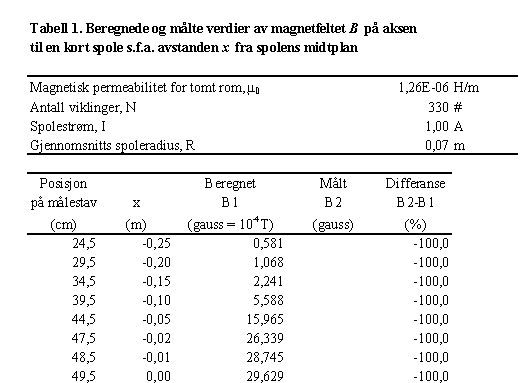
\includegraphics[scale=0.9]{fig/magnetfelt-tab1.png}

    \end{center}
    \caption{%
        Utdrag fra en Excel-tabell for magnetfelt på aksen til tynn spole.
    }
    \label{magnetfelt.tab1}
\end{figure}
%\emph{Hjelp:} Dersom f.eks. første tallinje i tabellen er skrevet inn på rad 14 og beregnet verdi er i kolonne 3 vil formelen som representerer likning \eqref{eq:kort.spole}  bli slik: \\[3mm]
%\verb" =(($E$4*$E$5*$E$6)/(2*$E$7))*((1+(B14/$E$7)^2)^(-1,5))*10000".
%\\[3mm]
%Verdien er multiplisert med \num{10000} slik at $B(x)$ vises i \si{\gauss} (\SI{e-4}{\tesla}), som er tallverdiene gaussmeteret viser. 

{\itsf 1B. Framstill resultatet i et kurvediagram.}

{\itsf Diskuter beregning av magnetfeltet til en kort spole når spolens utstrekning tas med i beregningen.}

Programmet eller regnearket i Excel kan også brukes for beregning av forventede magnetfeltstyrker som følge av Biot-Savarts \eqref{eq:Biot.Savart3} lov og påfølgende sammenligning med eksperimentelt målte magnetfeltstyrker i avsnitt \ref{ch.magnetfelt.eksperimentelt}.

{\itsf 1C. Inkluder en kolonne for målt verdi av $B$ og en kolonne for avvik mellom målt og beregnet verdi gitt i \si{\percent}, og forbered også til å vise avviket grafisk.} (Et forslag er gitt i tabellen i figur \ref{magnetfelt.tab1}.)

Ta en kontrollregning for hånd av en av de beregnede $B$. Sjekk utregnet differanse ved å sette inn den håndregnede verdien.

\vspace{4mm}

\emph{En nøtt for de som har god tid:}

Den virkelige spolen du skal bruke i oppgaven har 22 viklinger i 15 lag med en effektiv tråddiameter lik \SI{0,93}{\mm}, viklet med indre diameter lik \SI{126}{\mm} og ytre diameter lik \SI{154}{\mm}. 

{\itsf 2. Hvordan tror du at det virkelige magnetfeltet i nærheten av spolen vil avvike fra det magnetfeltet som beregnes fra likning \eqref{eq:kort.spole}?}
\footnote{TIPS: Se på utstrekningen av spolen som feil i $x$ og anslå tilsvarende feil $\Delta B$ i $B(x)$.}

{\itsf 3. Hvis du skulle ta hensyn til spolens utstrekning under beregningene av feltet hvordan ville du da gå fram?}\footnote{TIPS: Del spolen inn i f.eks. tre spoler med 110 viklinger hver og beregn feltet fra hver av spolene og superponer virkningen. Det beste du kan gjøre er å behandle hver vikling for seg, og i praksis betyr det integrasjon over hver vikling.}

\subsection{Helmholtzspoler}
%%%%%%%%%%%%%%%%%%%%%%%%%%%%%%%%%%%%%%%%%%%%%%%%%%%%%%

Såkalte Helmholtzspoler
%\footnote{Oppkalt etter Hermann Ludwig Ferdinand von Helmholtz (1821-1894), tysk medisiner og fysiker.} 
består av to identiske,  korte seriekoplede spoler satt opp parallelt på den samme aksen i en avstand $a$ som vist i figur \ref{magnetfelt.fig2}. Det aksiale magnetfeltet på aksen er gitt av likning \eqref{eq:kort.spole} for hver spole. Ifølge superposisjonsprinsippet finner vi det totale feltet i avstand $x$ fra midtplanet mellom spolene til å bli lik
%
\begin{equation}
    B_x (x) 
        = \frac{N \mu_0 I}{2 R} \qty[\qty(1 + \frac{(x - \flatfrac{a}{2})^2}{R^2})^{-3/2} 
            + \qty(1 + \frac{(x + \flatfrac{a}{2})^2}{R^2})^{-3/2}].
    \label{eq:Helmholtz}
\end{equation}
%
Her er spolenes gjennomsnittsradius lik $R$, strømmen gjennom spolene lik $I$ og vi har neglisjert utstrekningen av spolene.

Hvis du deriverer likning \eqref{eq:Helmholtz} mhp. $x$ finner du at ved $x = 0$ er $\dv*{B}{x} = \dv*[2]{B}{x} = \dv*[3]{B}{x} = 0$ når $a = R$. Dette betyr at når $a = R$ har du en geometri som gir deg et spesielt godt homogent magnetfelt i området mellom spolene. Slike Helmholtzspoler anvendes for å sette opp homogene magnetfelt i mange situasjoner.

\begin{figure}[!ht]
    \setlength{\unitlength}{0.6mm}
    \begin{picture}(120,80)(-50,20)
        \linethickness{0.5mm}
        \put(44,79){\makebox(0,0)[b]{\large$\bigodot$}}
        \put(44,19){\makebox(0,0)[b]{\large$\bigoplus$}}
        \put(40,19){\framebox(8,8)}%[20,20]{KRN}
        \put(40,79){\framebox(8,8)}%[20,60]{KRN}
        \put(104,79){\makebox(0,0)[b]{\large$\bigodot$}}
        \put(104,19){\makebox(0,0)[b]{\large$\bigoplus$}}
        \put(100,19){\framebox(8,8)}%[20,20]{KRN}
        \put(100,79){\framebox(8,8)}%[20,60]{KRN}
        \put(74,47){\line(0,1){6}} 
        \put(30,50){\vector(1,0){100}} %x-axis
        %\qbezier(128, 51)(129, 50.5)(130,50)
        %\qbezier(128, 49)(129, 49.5)(130,50)
        
        \qbezier(126, 51.5)(128, 50.8)(130,50)
        \qbezier(126, 49)(128, 49.5)(130,50)
        
        %\color{magenta}
        \put(44,60){\line(1,0){60}} 
        \qbezier(47, 61)(47, 61)(44,60)
        \qbezier(47, 59)(47, 59)(44,60)
        \qbezier(102, 61)(102, 61)(104,60)
        \qbezier(102, 59)(102, 59)(104,60)
        %%\color{yellow}
        \thinlines
        \put(39.7,27.8){\framebox(8.4,51)}%[20,60]{KRN}
        \put(99.7,27.8){\framebox(8.4,51)}%[20,60]{KRN}
        \put(134,48){\makebox(0,0)[b]{\large$x$}}
        \put(74,62){\makebox(0,0)[b]{\large$a$}}
        \put(74,40){\makebox(0,0)[b]{\large O}}
        \put(26,64){\makebox(0,0)[b]{\large$R$}}
        \put(68,20){\makebox(0,0)[b]{\small\sf Viklinger}}
        \put(32,50){\vector(0,1){32}}
        %%\color{magenta}
        \put(55,22){\vector(-1,-0){5}} 
    \end{picture}
    \caption{%
        Helmholtzspoler består av to tynne spoler i en gitt avstand $a$ mellom spolene.
    }
    \label{magnetfelt.fig2}
\end{figure}
Anta at du har Helmholtzspoler med $N = \SI{330}{\viklinger}$ på hver spole, $R = \SI{70}{\mm}$ og sender en konstant strøm $I = \SI{1,00}{\ampere}$ gjennom viklingene.

{\itsf 4A. Lag en tabell over magnetflukstettheten $B(x)$ på aksen til Helmholtzspolen i området $\SI{-20}{\cm} < x < \SI{20}{\cm}$ for hver av de tre forskjellige verdiene $a = R/2, R$ og $2R$.}

Et forslag til tabell er vist i figur \ref{magnetfelt.tab2}. 

\begin{figure}[!ht]
    \begin{center}
    %\vspace{25mm}
    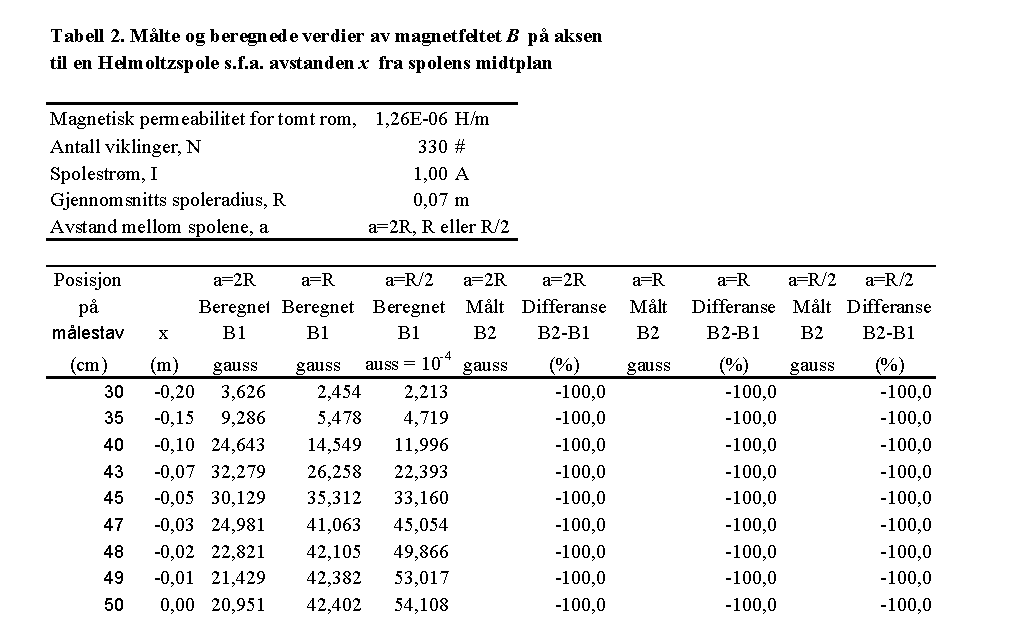
\includegraphics[width=0.8\textwidth]{fig/magnetfelt-tab2.eps}
    \end{center}
    \caption{%
        Utdrag fra tabell for magnetfelt på aksen til Helmholtzspoler.
    }
    \label{magnetfelt.tab2}
\end{figure}

{\itsf 4B. Framstill resultatet i et kurvediagram}

Regnearket skal også brukes for beregning av forventede magnetfeltstyrker som følge av Biot-Savarts lov \eqref{eq:Biot.Savart3}  og påfølgende sammenligning med eksperimentelt målte magnetfeltstyrker i avsnitt \ref{ch.magnetfelt.eksperimentelt}.

{\itsf 4C. Inkluder en kolonne for målt verdi av $B$ og en kolonne for avvik mellom målt og beregnet verdi gitt i \si{\percent} for $a = 2R$. Gjenta dette for de to andre verdiene av $a$. Forbered til å vise avviket grafisk.} (Et forslag er gitt i tabellen i figur \ref{magnetfelt.tab2}.)

Ta en kontrollregning for hånd av en av de beregnede $B$. Sjekk utregnet differanse ved å sette inn noen tenkte måleverdier.

\subsection{Anti-Helmholtzspoler}
%%%%%%%%%%%%%%%%%%%%%%%%%%%%%%%%%%%%%%%%%%%%%%%%%%%%%%

Anti-Helmholtzspoler består av to identiske, korte seriekoplede spoler satt opp parallelt på den samme aksen i en avstand $a$ som vist i figur \ref{magnetfelt.fig2a}, med ulik retning på magnetfeltet. Hvordan finner du feltet i denne konfigurasjonen?

\begin{figure}[!ht]
    \setlength{\unitlength}{0.6mm}
    \begin{picture}(120,80)(-50,20)
        \linethickness{0.5mm}
        \put(44,79){\makebox(0,0)[b]{\large$\bigodot$}}
        \put(44,19){\makebox(0,0)[b]{\large$\bigoplus$}}
        \put(40,19){\framebox(8,8)}%[20,20]{KRN}
        \put(40,79){\framebox(8,8)}%[20,60]{KRN}
        \put(104,79){\makebox(0,0)[b]{\large$\bigoplus$}}
        \put(104,19){\makebox(0,0)[b]{\large$\bigodot$}}
        \put(100,19){\framebox(8,8)}%[20,20]{KRN}
        \put(100,79){\framebox(8,8)}%[20,60]{KRN}
        \put(74,47){\line(0,1){6}} 
        \put(30,50){\vector(1,0){100}} %x-axis
        %\qbezier(128, 51)(129, 50.5)(130,50)
        %\qbezier(128, 49)(129, 49.5)(130,50)
        \qbezier(126, 51.5)(128, 50.8)(130,50)
        \qbezier(126, 49)(128, 49.5)(130,50)
        %\color{magenta}
        \put(44,60){\line(1,0){60}} 
        \qbezier(47, 61)(47, 61)(44,60)
        \qbezier(47, 59)(47, 59)(44,60)
        \qbezier(102, 61)(102, 61)(104,60)
        \qbezier(102, 59)(102, 59)(104,60)
        %%\color{yellow}
        \thinlines
        \put(39.7,27.8){\framebox(8.4,51)}%[20,60]{KRN}
        \put(99.7,27.8){\framebox(8.4,51)}%[20,60]{KRN}
        \put(134,48){\makebox(0,0)[b]{\large$x$}}
        \put(74,62){\makebox(0,0)[b]{\large$a$}}
        \put(74,40){\makebox(0,0)[b]{\large O}}
        \put(26,64){\makebox(0,0)[b]{\large$R$}}
        \put(68,20){\makebox(0,0)[b]{\small\sf Viklinger}}
        \put(32,50){\vector(0,1){32}}
        %%\color{magenta}
        \put(55,22){\vector(-1,-0){5}} 
    \end{picture}
    \caption{%
        Anti-Helmholtzspoler består av to tynne spoler i en gitt avstand $a$ mellom spolene.
    }
    \label{magnetfelt.fig2a}
\end{figure}

{\itsf 5A. Lag en tabell over magnetflukstettheten $B(x)$ på aksen til Anti-Helmholtzspolen i området $\SI{-20}{\cm} < x < \SI{20}{\cm}$ for hver av de tre forskjellige avstandene $a = R/2, R$ og $2R$.} 

{\itsf 5B. Fremstill resultatet i et kurvediagram.}

Regnearket skal også brukes for beregning av forventede magnetfeltstyrker som følge av Biot-Savarts lov \eqref{eq:Biot.Savart3}  og påfølgende sammenligning med eksperimentelt målte magnetfeltstyrker i avsnitt \ref{ch.magnetfelt.eksperimentelt}.

{\itsf 5C. Inkluder en kolonne for målte verdier av $B$ og en kolonne for avvik mellom målte og beregnede verdier gitt i \si{\percent} for $a = 2R$. Gjenta dette for de to andre verdiene av $a$. Forbered regnearket til å vise avviket grafisk.} (Et forslag er gitt i tabellen i figur \ref{magnetfelt.tab2}.)

Foreta en kontrollregning for hånd av en av de beregnede $B$. Sjekk utregnet differanse ved å sette inn det håndregnede verdien.

\subsection{Solenoide \label{ch.magnetfelt.solenoide}}
%%%%%%%%%%%%%%%%%%%%%%%%%%%%%%%%%%%%%%%%%%%%%%%%%%%%%%%%%

Magnetfeltet ved et punkt P på aksen til en solenoide kan finnes fra Biot-Savarts lov, og resultatet er
\begin{equation}
    B = \frac{N \mu_0 I} {2 \ell} \qty(\cos\theta_1 - \cos\theta_2),
    \label{eq:solenoide}
\end{equation}
hvor $\ell$ er lengden av solenoiden og vinklene $\theta_1$ og $\theta_2$ er definert i figur \ref{magnetfelt.fig3} eller analytisk:
\begin{equation}
    \cos \theta_1 = \frac{z}{\sqrt{z^2 + R^2}}, \qquad
    \cos \theta_2 = - \frac{\ell - z}{\sqrt{(\ell - z)^2 + R^2}},
\end{equation}
der $R$ = indre radius av solenoiden og $z$ er akseavstand fra venstre ende av solenoiden til punktet. Inni solenoiden er $\theta_1 \in \langle 0, \pi/2 \rangle$ og $\theta_2 \in \langle \pi/2, \pi \rangle$. Formelen gjelder også utenfor solenoiden.
%
\begin{figure}[!ht]
    \setlength{\unitlength}{0.9mm}
    \begin{picture}(120,80)(10,28)
        %\linethickness{0.5mm}
        \newsavebox{\OneTurn}
        \savebox{\OneTurn}{
        \put(44,80){\makebox(0,0)[b]{\large$\bigodot$}}
        \put(44,20){\makebox(0,0)[b]{\large$\bigotimes$}}
        }
        \multiput(0,20)(5.1,0){20}{\usebox{\OneTurn}}
        \put(44,72){\line(1,0){120}} 
        \put(44,72){\line(0,1){2}} %origin up
        \put(44,72){\line(0,-1){2}}%origin down
        %\put(104,72){\line(0,-1){2}}
        \put(104,64){\makebox(0,0)[b]{\large{P}}} 
        \put(44,64){\makebox(0,0)[b]{\large{O}}}  
        %\color{red}
        \qbezier(44, 102.5)(103, 72)(103,72)
        \qbezier(79.5, 102.5)(103, 72)(103,72)
        \qbezier(141, 102.5)(103, 72)(103, 72)
        %\color{black}
        \multiput(77,42)(0,3.4){18}{\line(0,1){2}}
        \multiput(81,42)(0,3.4){18}{\line(0,1){2}}
        \put(143,72){\vector(0,1){30}}%locating R
        \put(143,102){\vector(0,-1){30}}%locating R
        \put(146,88){\makebox(0,0)[b]{\large$R$}}
        \put(79,106){\makebox(0,0)[b]{\large$\rightarrow$}}
        \put(79,106){\makebox(0,0)[b]{\large$\leftarrow$}}
        \put(79,110){\makebox(0,0)[b]{$\dd{x}$}}
        \put(104,70){\vector(-1,0){25}}%locating x
        \put(79,70){\vector(1,0){25}}%locating x
        \put(90,66){\makebox(0,0)[b]{\large$x$}} 
        \qbezier(68, 72)(65, 80)(70,88)
        \put(64,80){\makebox(0,0)[b]{\large$\theta_1$}} 
        \qbezier(90, 72)(90, 77)(96,81)
        \put(90,80){\makebox(0,0)[b]{\large$\theta$}} 
        \qbezier(94, 72)(102, 82)(112,80)
        \put(104,82){\makebox(0,0)[b]{\large$\theta_2$}} 
        
        \put(44,52){\line(0,1){2}} %origin up
        \put(44,52){\line(0,-1){2}}%origin down
        \color{black}
        \put(44,52){\line(1,0){57}}
        \put(101,50.6){\makebox(0,0)[b]{\large$\succ$}}
        \put(90,54){\makebox(0,0)[b]{\large$z$}} 
        \put(44,30.4){\line(1,0){95.5}}
        %\color{magenta}
        \put(44.8,29){\makebox(0,0)[b]{\large$\prec$}}
        \put(138,29){\makebox(0,0)[b]{\large$\succ$}}
        %\put(44,101.6){\line(1,0){95.5}}
        \put(90,24){\makebox(0,0)[b]{\large$\ell$}} 
    \end{picture}
    \caption{%
        Solenoide. Vinkelen $\theta$ brukes ved utledning av magnetfeltet langs aksen, se teksten.
    }
    \label{magnetfelt.fig3}
\end{figure}

\emph{Vi spanderer et bevis for likning \eqref{eq:solenoide}:}  Vi har i likning \eqref{eq:Biot.Savart3} funnet magnetfelt på aksen i avstand $x$ fra en enkeltsløyfe. I en solenoide har vi mange sløyfer tett i tett, vi definerer strøm per lengdeenhet som $\flatfrac{I N}{\ell} = I n$, der $n$ er antall viklinger per lengde. Flukstetthet i et punkt P på aksen får da et bidrag fra den tynne strømsløyfa $\dd{I} = I n \dd{x}$ i posisjon $x$, og ifølge første del av likning \eqref{eq:Biot.Savart3} er flukstettheten lik
\begin{equation}
    \dd B 
        = \frac{\mu_0 \dd{I}}{4 \pi} \frac{2\pi R^2}{\qty(x^2 + R^2)^{3/2}}
        = \frac{\mu_0 I n}{2}  \frac{R^2}{ \qty( R^2 + x^2)^{3/2}} \dd{x} .
    \label{eq:solenoide2}
\end{equation}
%
Med $\theta$ som vinkelen i punktet P mellom solenoideaksen og periferien ved posisjon $x$ (figur \ref{magnetfelt.fig3}) ser vi at $\tan \theta = R / x$, og derivasjon av $x = R / \tan \theta$ gir 
\begin{equation}
    \dd{x} 
        = R \frac{-1}{\tan^2 \theta} \frac{1}{\cos^2\theta} \dd{\theta} 
        = -R \frac{1}{\sin^2\theta} \dd{\theta} .
\end{equation}
%
Vi merker oss at
\begin{equation}
    \sin^3 \theta = \frac{R^3}{(R^2 + x^2)^{3/2}},
\end{equation}
slik at 
\begin{equation}
    \dd{x} 
        = -R \frac{1}{\sin^3\theta} \sin\theta \dd{\theta}
        = -R \frac{(R^2 + x^2)^{3/2}}{R^3} \sin\theta \dd{\theta}
\end{equation}
og ved substitusjonen $\tan \theta = R / x$ i likning \eqref{eq:solenoide2} og innsetting av grenser $\theta_2$ (høyre ende, lavest $x$)  til $\theta_1$ (venstre ende, høyest $x$), vil vi få 
%
\begin{equation}
    B(x) 
        = -\frac{\mu_0 I n}{2} \int_{\theta_2}^{\theta_1} \sin \theta \dd{\theta}
        = \frac{\mu_0 I n}{2} (\cos \theta_1 - \cos \theta_2),
    \label{eq:solenoide3}
\end{equation}
som skulle vises. 
%Formelen gjelder også utenfor solenoiden med $\theta_1 > \pi/2$ utenfor høyre ende og $\theta_2 < \pi/2$ utenfor venstre ende

{\itsf 5. Hva  er uttrykket for magnetfeltet langt inne i solenoiden, og hva er det ved enden av solenoiden?}
\\
TIPS: Hva er $\theta_1$ og $\theta_2$ ved disse posisjonene?

Anta at du har en solenoide med  $N = \SI{397}{\viklinger}$, $\ell = \SI{420}{\mm}$, $R = \SI{50}{\mm}$ og strøm $I = \SI{1,00}{\ampere}$.

{\itsf 6A. Lag en tabell over magnetflukstettheten $B(z)$ på aksen til solenoiden i området $\SI{-10}{\cm} < z < \SI{50}{\cm}$ der $z = 0$ ved venstre kant av solenoiden.} % siunitx klarer ikke å merke tekstfamilien her...

%Hvis  $R \ll \ell$ og $x \neq 0$ og $x \neq \ell$ kan du ved rekkeutvikling finne at 
% Tatt ut denne approksimasjonen, da den ikke er god ved endene.
% Beregn forholdet B(X)/l på aksen -l \ t solenoiden i området2S:<J < x <s'o mm og framstill resultatet i et kurvediagram 

Et forslag til tabell er vist i figur \ref{magnetfelt.tab3}. 
%
\begin{figure}[ht]
    \begin{center}
    %\vspace{25mm}
    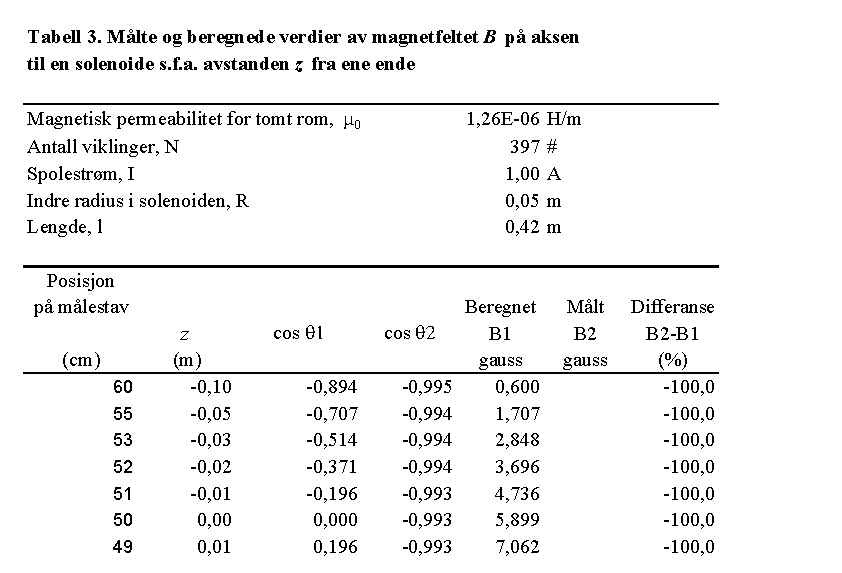
\includegraphics[width=0.7\textwidth]{fig/magnetfelt-tab3.eps}
    \end{center}
    \caption{%
        Utdrag fra tabell for magnetfelt på aksen til Helmholtzspoler.
    }
    \label{magnetfelt.tab3}
\end{figure}

{\itsf 6B. Framstill resultatet i et kurvediagram}

Regnearket skal også brukes for beregning av forventede magnetfeltstyrker som følge av Biot-Savarts lov \eqref{eq:Biot.Savart3}  og påfølgende sammenligning med eksperimentelt målte magnetfeltstyrker i avsnitt \ref{ch.magnetfelt.eksperimentelt}.

{\itsf 6C. Inkluder en kolonne for målt verdi av $B$ og en kolonne for avvik mellom målt og beregnet verdi gitt i \si{\percent}}. (Et forslag er gitt i tabellen i figur \ref{magnetfelt.tab3}.)

\subsection{Dataanalyse i Python}
De foregående oppgavene kan for eksempel gjøres i Python. Det er hensiktsmessig å lagre dataene i tekstfiler. Her bruker vi kommaseparerte filer som vist under.

\begin{verbatim}
# Posisjon (m), B-felt (Gauss)
0.245,0.0
0.295,0.623
...
\end{verbatim}

Her representerer første kolonne \emph{Posisjon på målestav}, og den andre kolonnen representerer \emph{Målt B2} i figur \ref{magnetfelt.tab1}. De resterende kolonnene kan man beregne i Python. For å lese inn dataene lager vi følgende kode:

\begin{minted}[bgcolor=bg]{python}
# -*- coding: utf-8 -*-
import numpy as np


def main():
    filnavn = 'kort_spole.csv'
    data = np.loadtxt(filnavn, delimiter=',')
    xe = data[:, 0]
    Be = data[:, 1]

if (__name__ == '__main__'):
    main()
\end{minted}

I \texttt{main}-funksjonen leses tekstfilen \emph{kort\_spole.csv}. Posisjonsdataene, som ligger i første kolonne, legges i variabelen \texttt{xe} og dataene for det målte magnetfeltet lagres i variabelen \texttt{Be}.

Det neste vi må gjøre er å implementere en funksjon som beregner magnetfeltet i henhold til ligning \eqref{eq:kort.spole}. Dette kan vi gjøre slik:

\begin{minted}[bgcolor=bg]{python}
def B_felt_kort_spole(x):
    prefaktor = N*mu_0*I0/(2*R)
    return prefaktor*(1.0 + (x/R)**2)**(-1.5)
\end{minted}

For å plotte resultatet for det beregnede feltet legger vi til noen linjer i \texttt{main}-funksjonen. Vi må også definere noen parametre som brukes i utregningen. Hele programmet blir da seende slik ut:

\begin{minted}[bgcolor=bg]{python}
# -*- coding: utf-8 -*-
import numpy as np
from matplotlib import pyplot as plt


N = 330                 # [] antall viklinger
I0 = 1.0                # [A] strøm 
mu_0 = 4.0*np.pi*1e-7   # [H/m] permeabilitet i tomt rom
R = 0.07                # [m] radius
x0 = 0.400              # [m] sentrum av spolen

def B_felt_kort_spole(x):
    prefaktor = N*mu_0*I0/(2*R)
    return prefaktor*(1.0 + (x/R)**2)**(-1.5)
    
def main():
    filnavn = 'kort_spole.csv'
    data = np.loadtxt(filnavn, delimiter=',')
    xe = data[:, 0] - x0    # posisjon, sentrert rundt x0
    Be = data[:, 1]         # måledata 
    
    # Beregn B-feltet
    xb = np.linspace(xe[0], xe[-1], 100)    # flere datapunkter
    Bb = B_felt_kort_spole(xb)*1e4          # beregnet B-felt (Gauss)
    
    # Plot resultatene
    plt.plot(xb, Bb, label='Beregnet')
    plt.plot(xe, Be, '.', label='Måledata')
    plt.xlabel('Avstand fra senter av spolen (m)')
    plt.ylabel('Magnetfelt (Gauss)')
    plt.legend()
    plt.show()
    
if (__name__ == '__main__'):
    main()
\end{minted}

Man kan nå lage flere funksjoner for å plotte resultatene for en Helmholtzspole og en solenoide. Husk at det ofte lønner seg å dele programmet opp i mindre funksjoner. Det gjør at koden blir lettere å lese, men også at man kan gjenbruke mye av koden til andre formål. Man kan finne mer eksempler om plotting her: \url{https://nbviewer.jupyter.org/urls/www.numfys.net/media/notebooks/basic_plotting.ipynb}. 

\subsection{Halleffektprobe}
%%%%%%%%%%%%%%%%%%%%%%%%%%%%%%%%

Når elektroner beveger seg med hastighet $\va*{v}$ i en halvleder som befinner seg i et magnetfelt $\va*{B}$ som vist i figur \ref{magnetfelt.fig4}, vil elektronene bøye av til den ene siden. Avbøyningen er gitt ved Lorentzkraften $\va*{F} = q(\va*{v} \cross \va*{B})$, der $q = -e$ for elektroner.  

\begin{figure}[!ht]
    \setlength{\unitlength}{0.8mm}
    \begin{picture}(120,80)(-10,20)
        \put(50,30){\framebox(40,10)}%lower rectangle
        \put(90,70){\dashbox{0.2}(40,10)}%upper rectangle
        %\qbezier(70, 55)(70,80)(120,100)
        %\qbezier(50, 30)(58,50)(66,70)
        \put(50,30){\line(1,1){40}}
        \put(50,40){\line(1,1){40}}
        \put(90,30){\line(1,1){40}}
        \put(90,40){\line(1,1){40}}
        \put(70,55){\tiny$\bullet$}%left side
        \multiput(70,55.5)(-2,0){2}{\line(-1,0){1}}
        \multiput(67,55.5)(0,2){2}{\line(0,1){1}}
        \put(67,57){\line(0,1){35}}
        \put(110,55){\tiny$\bullet$}%right side
        \put(110.5,55.5){\line(1,0){25}}
        %\color{green}
        \put(136,55.5){\line(0,1){36.5}}
        \put(136,55.5){\line(0,1){36.5}}
        %\put(136,55.5){\line(0,1){36.5}}
        %\put(67,92){\line(1,0){75}}
        \put(67,92){\line(1,0){28}}
        \put(95,91.5){\tiny$\bullet$}     %left top
        \put(99,91.5){\large$V_\text{H}$} 
        \put(108,91.5){\tiny$\bullet$}    %right top
        %\color{red}
        \put(136,92){\line(-1,0){28}}
        \put(69.5,35){\tiny$\bullet$}%front
        \put(109.5,75){\tiny$\bullet$}%back
        %\put(70,35){\line(1,1){60}}
        \put(60,25){\line(1,1){10}}    %Current in
        \put(55,20){\Huge\vector(1,1){6}}   %Current in arrow
        \put(110,75){\vector(1,1){12}} %Current out
        \put(90,56){\vector(1,0){10}}
        \put(90,56){\vector(-1,-1){7}}
        \put(95,50){\footnotesize$\va*{F}$}
        \put(80,45){\footnotesize$\va*{v}$}
        \put(96,63){$\va*{B}$}
        \put(85,55){\footnotesize$q$}
        \put(89.25,55.25){\tiny$\bullet$}
        \put(95,58){\vector(0,1){9}}
        \put(96,63){$\va*{B}$}
        \put(43,32){\Huge$\updownarrow$}
        \put(40,33){\large$d$}
        \put(60,20){\large$I$}
        \put(49,24.5){\Huge$\longleftarrow$}
        \put(68,25){\large$b$}
        \put(73,24.5){\Huge$\longrightarrow$}
    \end{picture}
    \caption{\small\sf Halleffekt i en halvlederprobe. Strøm $I$ påtrykkes mellom de to minste endevegger.}
    \label{magnetfelt.fig4}
\end{figure}

%\begin{figure}[h]
%\begin{center}
%%\vspace{25mm}
%\includegraphics[width=90mm]{fig/magnetfelt.fig4.eps}
%\end{center}
%\caption{\sf Halleffekt i en halvlederprobe. Strøm $I$ påtrykkes mellom de to minste endevegger.}
%\label{magnetfelt.fig4}
%\end{figure}

Lorentzkraften virker normalt på strømretningen og normalt på $B$ og avbøyningen på grunn av denne fører til at elektronkonsentrasjonen blir sterkere mot den ene veggen av halvlederen. Det bygger seg altså opp et elektrisk felt $\va*{E}$ i lederen med samme retning som Lorentzkraften, og dette feltet gir en tilleggskraft $\va*{F} = q \va*{E}$ på elektronene. Det vil raskt oppstå en likevekt der elektrostatisk kraft og Lorentzkraft er like store slik at 
\begin{equation}
    \va*{F} =  q \va*{E} + q(\va*{v} \cross \va*{B}) = \va*{0}
    \quad \Rightarrow \quad
    \va*{E} = -\va*{v} \cross \va*{B} .
\end{equation}

Farten $v$ til elektronene gjennom halvlederen er bestemt av strømmen ved uttrykket $I = nqvA$, hvor $n$ er tettheten av elektroner og $A = bd$ er tverrsnittet i lederetningen. Dette gir 
\begin{equation}
    v = \frac{I}{A} \frac{1}{nq} 
        = \frac{I}{bd} R_\text{H},
\end{equation}
der vi har definert Hallkonstanten $R_\text{H} = 1/nq$.  

Med $b$ lik bredden på proben vil spenningen $V_\text{H} = E b$ dannes over sideveggene. Hvis vi ser bort fra fortegn og bruker at $\va*{v} \perp \va*{B}$ får vi følgende uttrykk for Hallspenningen $V_\text{H}$:

\begin{equation}
    V_\text{H} = Eb
        =  vBb 
        = \frac{R_\text{H} I}{d} B,
    \label{eq:Hall}
\end{equation}

der altså $d$ er tykkelsen av Hallproben som magnetfeltet $B$ virker over. Hallkonstanten $R_\text{H}$ og $d$ er konstanter for en gitt probe og strømmen $I$ holdes konstant. Den magnetiske flukstettheten $B$ normalt på proben vil da være proporsjonal med Hallspenningen $V_\text{H}$ som måles med et voltmeter. 

%\vspace{1cm}
\begin{figure}[htb]
    \begin{minipage}[b]{0.4\linewidth}
    \centering
    \begin{overpic}[scale=0.5]{fig/HallAx.eps}
        \put(-12, 14){\large$1$}
        \put(115,14){\large$\va*{B}$}
        \put(95,14){\Huge$\rightarrow$}
        \label{fig:figure1}
    \end{overpic}
    \end{minipage}%
    %
    \hspace{1.5cm}%
    %
    \begin{minipage}[b]{0.4\linewidth}
    \centering
    \begin{overpic}[scale=0.5]{fig/HallTr.eps}
        \put(-12, 14){\large$2$}
        \put(100, 14){\Huge$\downarrow$}
        \put(112, 14){\large$\va*{B}$}
    \end{overpic}
    \label{fig:figure2}
    \end{minipage}
    \caption{%
        Probegeometrier: (1) Aksial probe, (2) transversal probe.
    }
    \label{magnetfelt.fig8}
\end{figure}

%%%%%\vspace{2cm}

Halleffekten anvendes bl.a. i gaussmetre for måling av magnetfelt. Et Halleffekt-gaussmeter vil essensielt bestå av en strømkilde som gir en konstant strøm $I$ gjennom en probe,  og et voltmeter. Proben plasseres i magnetfeltet som skal måles. Gjennom en kalibreringsprosess kan sammenhengen mellom målt Hallspenning og magnetfelt etableres og utlesningsenheten for spenning graderes direkte i $\si{\tesla} = \si{\weber/\square\m}$ eller $\si{gauss} = \SI{e-4}{\tesla}$.

I praksis er utstrekningen til en Hallprobe av størrelsesorden noen \si{\square\mm}. To forskjellige probegeometrier er vanlige: transversale prober og aksiale prober, som vist i figur \ref{magnetfelt.fig8}.

Typisk verdi for elektrontettheten i en dopet halvleder er $n = \SI{e20}{\elektroner/\m\cubed}$. Til sammenlikning har kobber $n = \SI{e28}{\elektroner/\m\cubed}$. I våre gaussmetre er $I = \SI{20}{\milli\ampere}$ og $d = \SI{1,0}{\mm}$. Anta at magnetfeltet varierer fra 1 til \SI{100}{\gauss}.

{\itsf 7A. Hvilket måleområde må gaussmeterets voltmeter ha for å måle i dette magnetfeltområdet? (Anta at $n = \SI{e20}{\elektroner/\m\cubed}$.)

7B. Hvorfor tror du at halvledere blir brukt i magnetfeltprober? Begrunn hvorfor f.eks. kobber ikke vil være et egnet materiale.
 
7C. Begrunn også hvorfor en isolator ikke vil være et egnet materiale i en magnetfeltprobe.
}

\subsection{Magnetiske strøfelt}

I laboratoriet er det magnetiske strøfelt som danner en bakgrunn som kan forstyrre magnetfeltmålinger. Strøfeltene har tre hovedkilder: 
\vspace{-4mm}
\begin{itemize}
    \item jordmagnetfeltet,
    \item magnetfelt fra magnetiske materialer i bygningskonstruksjoner og inventar,
    \item induserte magnetfelt fra bl.a. \SI{230}{\volt} nettledninger.
\end{itemize}

Jordmagnetfeltet, som er konstant og av størrelsesorden \SI{1}{\gauss}, antas å stamme fra konveksjonsstrømmer av elektriske ladninger i jordas flytende kjerne. Anta at det midt i jordas indre ligger en strømsløyfe vinkelrett på jordas rotasjonsakse. La strømsløyfas radius være $R = R_\text{j}/4$, hvor $R_\text{j} = \SI{6371}{\km}$ er jordradien. Aksialkomponenten til magnetfeltet i posisjon $x$ på aksen til en slik strømsløyfe er gitt ved likning \eqref{eq:Biot.Savart3}.

{\itsf 8. Hvor stor må strømmen i sløyfa være for at magnetfeltet på jordoverflata ved polen ($x = R_\text{j}$) skal være lik \SI{1}{\gauss}? }

%{\itsf 8B. Er det en god antakelse å bruke $\mu_0$ som permeabilitet i jordas indre? }

Bidrag til strømagnetfeltet fra bygningen og inventaret vil avhenge av bygnings- og konstruksjonsmaterialene som er brukt. Dere skal vurdere bidragene til dette i laboratoriet gjennom egne målinger.

Bidrag til strøfeltet fra strømmene i ikke-skjerma ledninger kan estimeres ved å beregne feltet satt opp av en lang rett leder som fører strømmen $I$. Asimutalkomponenten av magnetfeltet i en avstand $r$ fra en lang leder kan finnes fra\footnote{Utledning f.eks. i \cite{lillestol}, Kap. 23.5.} Biot-Savarts lov \eqref{eq:Biot.Savart2}
\begin{equation}
    B_\theta (r) = \frac{\mu_0 I}{2\pi r} .
\end{equation}

{\itsf 9. Hvor stor er den magnetiske flukstetthet i en avstand \SI{5}{\cm} fra en lang \SI{230}{\volt} nettledning pga. en strøm \SI{1}{\ampere} i denne ledningen?}

\subsection{Magnetfeltfritt rom \label{ch.mymetall}}
%%%%%%%%%%%%%%%%%%%%%%%%%%%%%%%%%%%%%%%%%%%%%%%%%%%%%%%

Det permanente magnetfeltet på jordoverflata fører til problemer med nulling av gaussmetre. Magnetfelt kan imidlertid skjermes ved å bruke materialer med høy permeabilitet. Rent jern kan brukes. Det finnes også spesielle legeringer som har enda høyere permeabilitet $\mu$ og dermed skjermer enda bedre. Et eksempel er mymetall\footnote{Mymetall er en legering av \SI{77}{\percent} nikkel, \SI{15}{\percent} jern pluss noe kobber og molybden.  Navnet har det fått pga. svært høy verdi for magnetisk permeabilitet, $\mu$.}. Gaussmetre nulles vanligvis ved å stikke gaussmeterproben inn i et kammer som skjermer den fra jordmagnetfeltet under nullingen. 

%{\itsf 10. Hvordan ville du utforme et kammer av mymetall, med et lite hull i enden, på en slik måte at det inne i kammeret ble fritt for magnetfelt? }
%\footnote{TIPS: Ta ved utformingen av kammeret hensyn til at magnetiske feltlinjer må alltid følge en sluttet bane.}

\section{Eksperimentelt \label{ch.magnetfelt.eksperimentelt}}
%%%%%%%%%%%%%%%%%%%%%%%%%%%%%%%%%%%%%%%%%%%%%%%%%%%%%%%%%%%%%%%%%%%%%%%%%%%%%%

%%%%%%%%%%%%%%%%%%%%%%%%%%%%%%%%%%%%%%%%%%%%%%%%%%%%%%%%%%%%%%%%%%%%%%%%%%%%%%
\subsection{Apparatur}
%%%%%%%%%%%%%%%%%%%%%%%%%%%%%%%%%%%%%%%%%%%%%%%%%%%%%%%%%%%%%%%%%%%%%%%%%%%%%%

Eksperimentet bruker PASCOs system for datalogging (Capstone) med grensesnitt og sensorer for magnetfelt og posisjon.
Følgende instrumenter inngår i oppstillingen:
\vspace{-4mm} 
\begin{itemize}
    \item \textbf{Grensesnitt.} PASCO 550 Universal Interface.
    \item \textbf{Magnetfelt sensor.} PASCO Magnetic Field Sensor CI-6520A.\\
    Måleområde: \SI{0,01}{\G}--\SI{100}{\kilo\G}.\\
    Oppløsing: \SI{50}{\milli\G}.
    Accuracy: 10\% of reading
    \item \textbf{Nullfeltkammer.} PASCO Zero Gauss Chamber EM-8652. 
    \item \textbf{Posisjonssensor.} PASCO Rotary Motion Sensor PS-2120A. \\
    Oppløsning: \SI{0,09}{\degree}. \\
    Radier på de tre trinsene: \SI{10}{\mm}, \SI{29}{\mm}, \SI{48}{\mm}.
    \item \textbf{Korte spoler.} 330 viklinger, 22 viklinger/lag $\cross$ 15 lag\\
    Indre diameter \SI{126}{\mm}, ytre diameter \SI{154}{\mm}.\\
    Tråd: lakkisolert kobber, diameter \SI{0,75}{\mm}, maksimum spolestrøm: \SI{1,0}{\ampere}. 
    \item \textbf{Solenoide.} 368 viklinger, lengde $\sim \SI{400}{\mm}$, indre diameter \SI{100}{\mm}.\\
    Tråd: lakkisolert kobber, diameter \SI{1,0}{\mm}, maksimum solenoidestrøm \SI{1,0}{\ampere}. 
    \item \textbf{Multimeter.} Escort Mod. EDM 168A, eller tilsvarende. 
    %\item \textbf{Datamaskin} med printer.
    \item \textbf{Diverse utstyr:} Metermål, skrujern. 
    \item \textbf{Kraftforsyning.} Mascot Type 719. Område: 0-\SI{30}{\volt}, \SI{30}{\milli\ampere}-\SI{2}{\ampere}. \label{magnetfelt.kraftforsyning}
    %\\[1mm]
    Dette er en kombinert strømstyrt/spenningstyrt kraftforsyning. Dvs.\ den kan forsyne en konstant strøm eller en konstant spenning, opp til en viss maksimal belastning. Boksen har to justeringsknapper, en for spenning merket "$0 \rightarrow \SI{30}{\volt}$" og en for strøm merket "$\SI{30}{\milli\ampere} \rightarrow \SI{2}{\ampere}$".
    %\\[1mm]
    \textbf{Strømstyrt kraftforsyning (strømkilde)} har vi dersom spenningsjusteringen stilles til maksimalt. Strømmen reguleres med strømjusteringsknappen. 
    %\\[1mm]
    \textbf{Spenningstyrt kraftforsyning (spenningskilde)} har vi dersom strømjusteringen stilles til maksimalt. Spenningen reguleres med spenningjusteringsknappen. 
    %\\[1mm]
    Dersom boksen brukes strømstyrt vil den maksimale strømmen \SI{2}{\ampere} kunne gis til en ekvivalent utgangsmotstand på maksimalt $R = U/I = \SI{30}{\volt} / \SI{2}{\ampere} = \SI{15}{\ohm}$. Boksen har også en knapp merket "range" som kan begrense maksimal spenning til \SI{15}{\volt} istedenfor standard \SI{30}{\volt}. Dersom \SI{15}{\volt} velges vil maksimal utgangsmotstand være $R = U/I = \SI{15}{\volt} / \SI{2,0}{\ampere} = \SI{7,5}{\ohm}$. Ved høyere utgangsmotstand vil utgangsspenningen holdes på maksimal verdi og strømmen bli lavere.
    %\\[1mm]
    Tilsvarende maksimalregulering er det ved spenningsstyrt kraftforsyning. \SI{30}{\volt} maksimalspenning kan gis ned til en motstand på $R = U/I = \SI{30}{\volt} / \SI{2,0}{\ampere} = \SI{15}{\ohm}$. Ved lavere motstand vil forsyningen ikke kunne gi nok strøm slik at spenningen vil falle.
\end{itemize}

\subsection{Kaliberering av Hallprobe}
%%%%%%%%%%%%%%%%%%%%%%%%%%%%%%%%%%%%%

Det er vanskelig å produsere Hallprober med nøyaktig like Hallkonstanter. Hallspenningen som oppstår ved et gitt magnetfelt og strøm vil derfor kunne variere litt fra probe til probe. For å kunne bruke flere prober til samme gaussmeter har ofte hver probe tilordnet et kalibreringsnummer som brukes for å justere forsterkningen til gaussmeterets voltmeter slik at meteret viser riktig magnetfelt. PASCOs sensorer er justert og en kaliberering trengs normalt ikke. Før bruk må sensoren nullstilles. 

\textbf{Nullstillingsprosedyre:}
\vspace{-5mm}
\begin{itemize}
    \item Sett områdeknappen på sensoren i stilling 1x og axial.
    \item Før proben inn i nullfeltkammeret og trykk på nulljusteringsknappen.
%\item Gjenta prosedyren hvis område endres.
%\item Sett områdeknappen i stilling 1 K.
\end{itemize}

%\textbf{MERK:} Før gaussmeteret er klart til bruk må det varmes opp i 15--20 min. Under oppvarmingen vil kalibreringen og nullstillingen drive. Før du begynner å ta nøyaktige målinger må du derfor gjenta kalibrering og nullstilling. \\
\textbf{MERK:} Når du skifter måleområde må du foreta ny nullstilling!

\textbf{Enheter og fortegn for Hallproben:}
\vspace{-5mm}
\begin{itemize}
    \item Meteret viser den magnetiske flukstettheten, $B$, i den enhet du velger i Capstone.
    \item Gaussmeteret viser \textbf{positivt} fortegn når feltlinjene har retning \textbf{inn} av den sylindriske tuppen på proben.
\end{itemize}

\subsection{Magnetiske strøfelt}
%%%%%%%%%%%%%%%%%%%%%%%%%%%%%%%%%%%%%

Oppgave:\\
{\itsf Undersøk de magnetiske strøfeltene i laboratoriet og svar på følgende spørsmål:}
\vspace{-5mm}
\begin{itemize}
    \item Hvordan stemmer den målte retningen av jordmagnetismen med antatt retning for vår breddegrad?\footnote{Den magnetiske nordpolen ligger i nærheten av den geografiske sydpolen. Magnetiske feltlinjer er lukkede kurver og har retning fra magnetisk nordpol til sydpol ytre sett og fra sydpol til nordpol inni magneten.}
    \item Sammenlikn resultatene med resultater fra de andre gruppene. Er det variasjon av den målte jordmagnetismen innenfor laboratoriet?
    \item Vil magnetfeltet fra jernet i laboratoriebordene kunne forstyrre målingene?
\end{itemize}

%Som allerede nevnt er det strøfelt fra jordmagnetismen, elektriske ledninger, jernholdige materialer som laboratoriebenker etc.}

%Du bør sette gaussmeteret i stilling 10x for disse målingene (og husk å nullstille på ny!)

\subsection{Statistisk feil i målinger}
%%%%%%%%%%%%%%%%%%%%%%%%%%%%%%%%%%%%%

Avlesing av magnetfeltstyrker fra Hallproben vil gi et noe varierende resultat. Dette kan du bruke til å finne den statistiske feilen.

Oppgave:\\
{\itsf Undersøk statistisk feil i målinger:}
\vspace{-5mm}
\begin{itemize}
    \item Koble inn sensorene i PASCOs grensesnitt og grensesnittet til datamaskinen. Start Capstone og gjør klar til datasampling.
    \item Nullstill og sample data i \SI{10}{\s}. Marker data og foreta en statistisk analyse med innebygd funksjonalitet i Capstone. Hva blir dataenes standardavvik? Hvilke standardavvik får du om du sampler i \SI{1}{\s} og \SI{100}{\s}? Hvor mange samples bør du bruke?
    \item Bruk standardavviket som feil i dine data fra Hallproben.
\end{itemize}

\subsection{Magnetfelt i kort spole}
%%%%%%%%%%%%%%%%%%%%%%%%%%%%%%%%%%%%%

Oppgave:\\
{\itsf Kartlegg magnetfeltet på aksen til en kort spole sfa. avstanden fra spolen.}
 
%Drøfting av måleprosedyren: 

For å måle magnetfeltet kan du enten holde spolen fast og flytte Hallproben eller du kan sette Hallproben fast og flytte spolen.
Hvilken av disse er best å bruke? Motivere!
%I våre eksperimenter er siste løsning den beste fordi vi da unngår korrigering av gaussmeteravlesningene pga. det varierende strøfeltet langs spoleaksen. Når Hallproben sitter fast vil strøfeltet rundt proben være konstant og kan nulles ut vha. gaussmeterets nullstilling og feltet fra spolen kan følgelig leses direkte. 

\textbf{Framgangsmåte:}
\vspace{-5mm}
\begin{itemize}
    \item Monter rotasjonssensoren på stativet. 
    \item Kople sensorene inn i grensesnittet og grensesnittet i datamaskinen. Start Capstone og gjør klar til datasampling. 
    \item Monter en kort spole på den bevegelige vogna.
    \item Juster magnetfeltssensorens posisjon slik at den ligger på spoleaksen. Bruk vater.
    %\item Klargjør kraftforsyningen. 
    %Sjekk at den er avslått og justeringsknappene for strøm og spenning er skrudd helt ned.
    %Innstill til strømstyrt kraftkilde (se beskrivelsen av kraftforsyning side \pageref{magnetfelt.kraftforsyning}). 
    %\item Klargjør multimeteret.\\
    %Sjekk at det er avslått, sett AC/DC innstillingen i stilling DC og funksjonsvelgeren for strømmåling i området 0 - 20 A.\\
    %VIKTIG: Bruk kontakten for tilkopling av likestrøm i området 0 - 20 A. %Bruk denne, ellers går mulitmeterets sikring umiddelbart.
    \item Kople opp spolekretsen som vist i figur \ref{magnetfelt.fig6}.\\
    VIKTIG: Kraftforsyningen skal være avslått under oppkoplingen. Velg strømmåling både på kraftforsyningen og multimeteret. Bruk 10A-inngangen på multimeteret.
    \\
    -- Be labveilederen om å godkjenne oppkoplingen.
    \item Nullstill magnetfeldsensoren. (Det er sikrest å bryte spolestrømkretsen under nullingen.)  
    \begin{figure}[!ht]
        \setlength{\unitlength}{0.8mm}
        \begin{picture}(120,80)(-30,0)
        
            \put(30,5){\line(1,0){88}}
            \put(118,5){\line(0,1){23}}
            \put(30,5){\line(0,1){14}}
            \qbezier(118, 28)(124, 28)(129,35)
            \qbezier(129, 35)(132, 40)(132,45)
            \qbezier(132,45)(132, 52)(125,58)
            \qbezier(125,58)(117, 63)(108,58)
            \qbezier(108,58)(102, 54)(101,45)
            \qbezier(101,45)(101, 38)(105,34.5)
            \qbezier(105,34.5)(109, 30)(115,30)
            %\color{red}
            \qbezier(115,30)(126, 31)(129,40)
            \qbezier(129,40)(132, 55)(118,58)
            \qbezier(118,58)(105, 59)(103,45)
            \qbezier(103,45)(102, 35)(114,32)
            \put(120,10){\Large$\uparrow$}%
            \put(125,10){\large$I$}%
            
            \put(50,15){\framebox(15,25)}%Multimeter
            \put(52.5,32){\framebox(10,5)}%Multimeter display
            \put(56,20){\circle{3}}%
            \put(55,18.7){\small$\bullet$}%
            \put(62,20){\circle{3}}%
            \put(60.7,18.7){\small$\bullet$}%
            
            \put(61.5,20){\line(1,0){53}}
            \put(114,32){\line(0,-1){12}}
            \put(52,16){\tiny\sf COM}%
            \put(60,16){\tiny\sf 10A}% 
            \put(45,45){\sf Multimeter}%
            %\color{red}
            \put(114,20){\circle{3}}%
            \put(113,18.7){\small$\bullet$}%
            \put(118,20){\circle{3}}%
            \put(116.7,18.7){\small$\bullet$}%
            \put(105,22){\sf Bl\aa}%
            \put(119,22){\sf R\o d}%
            %\color{green}
            %%%%%%%%%Mascot begins
            \put(20,15){\framebox(20,34)}%Mascot
            \put(22,40){\framebox(9,5)}%Mascot
            \put(35,43){\framebox(3,5)}%Mascot
            \put(35,36){\framebox(3,5)}%Mascot
            \put(35,29){\framebox(3,5)}%Mascot
            \put(30,20){\circle{3}}%
            \put(28.8,18.7){\small$\bullet$}%
            \put(36,20){\circle{3}}%
            \put(34.6,18.7){\small$\bullet$}%
            \put(28,23){$+$}%
            \put(34,23){$-$}%
            \put(35,20){\line(1,0){22}}%Mascot-to-Multimeter
            \put(23,54){\sf Mascot}%
            %%%%%%%%%Mascit ends
            %\put(90,70){\dashbox{0.2}(40,10)}%upper rectangle
        \end{picture}
        \caption{%
            Spolekrets. Mascot kraftforsyning, multimeter og spolen er vist. Merk deg vikleretningen for spolen, spolen er sett mot siden med koplingsbøssingene.
        }
        \label{magnetfelt.fig6}
    \end{figure}

    \item Mål magnetfeltet $B(x)$ langs aksen av spolen sfa. avstanden $x$ fra spolens midtplan
    %\footnote{TIPS: Definer spolens midtplan på følgende måte: Finn magnetfeltets maksimumsverdi. Finn to posisjoner på hver side av spolens midtplan hvor magnetfeltene er like og ligger ca \SI{5}{\percent} under maksimumsverdien. Midtplanet ligger midt i mellom disse to posisjonene.}
    Husk: maksimal spolestrøm er \SI{1,0}{\ampere}; Kontroller at du ikke har en drift i målingen.
\end{itemize}
 
Analyser resultatene og sammenligner målt og beregnet verdi. Skriv ut tabell og graf og lim inn i journalen.

\subsection{Magnetfelt i Helmholtzspole}
%%%%%%%%%%%%%%%%%%%%%%%%%%%%%%%%%%%%%

Oppgave:\\
{\itsf Kartlegge magnetfeltet på aksen mellom to korte spoler sfa. avstanden fra spolens midtplan og avstanden mellom spolene.}
 
\textbf{Framgangsmåte:}
\vspace{-5mm}
\begin{itemize}
    \item Monter på den bevegelige vogna to korte spoler i en avstand $a = R$ fra midtplan til midtplan .
    \item Mål magnetfeltet $B(x)$ langs spoleaksen som funksjon av avstanden $x$ fra midtplanet mellom spolene med f.eks. $I = \SI{1,00}{\ampere}$ og legg resultatene etter hvert inn i regnearktabellen for Helmholtzspolen. Mål et stykke utenfor enden av spolen.
    \item Gjenta målingen med spoleavstander $a = 2R$ og $a = R/2$.
    \item Analyser resultatene og sammenligner målt og beregnet verdi. Skriv ut tabell og graf og lim inn i journalen.
\end{itemize}

\begin{figure}[!ht]
    \setlength{\unitlength}{0.8mm}
    \begin{picture}(120,80)(-10,0)
        \newsavebox{\OneCoil}
        \savebox{\OneCoil}(60,60)[l]{
        %\put(30,5){\line(1,0){88}}
        %\put(118,5){\line(0,1){23}}
        \put(114,32){\line(0,-1){26.5}}
        \put(118,28){\line(0,-1){37.5}}
        
        %\put(30,5){\line(0,1){14}}
        \qbezier(118, 28)(124, 28)(129,35)
        \qbezier(129, 35)(132, 40)(132,45)
        \qbezier(132,45)(132, 52)(125,58)
        \qbezier(125,58)(117, 63)(108,58)
        \qbezier(108,58)(102, 54)(101,45)
        \qbezier(101,45)(101, 38)(105,34.5)
        \qbezier(105,34.5)(109, 30)(115,30)
        %\color{red}
        \qbezier(115,30)(126, 31)(129,40)
        \qbezier(129,40)(132, 55)(118,58)
        \qbezier(118,58)(105, 59)(103,45)
        \qbezier(103,45)(102, 35)(114,32)
        }
        %%Single Coil begins
        \put(30,5){\line(1,0){123}}
        %\put(118,5){\line(0,1){23}}
        \put(118,20){\line(1,0){31}}
        \put(118,28){\line(0,-1){7}}
        
        \put(30,5){\line(0,1){14}}
        \qbezier(118, 28)(124, 28)(129,35)
        \qbezier(129, 35)(132, 40)(132,45)
        \qbezier(132,45)(132, 52)(125,58)
        \qbezier(125,58)(117, 63)(108,58)
        \qbezier(108,58)(102, 54)(101,45)
        \qbezier(101,45)(101, 38)(105,34.5)
        \qbezier(105,34.5)(109, 30)(115,30)
        %\color{red}
        \qbezier(115,30)(126, 31)(129,40)
        \qbezier(129,40)(132, 55)(118,58)
        \qbezier(118,58)(105, 59)(103,45)
        \qbezier(103,45)(102, 35)(114,32)
        \put(90,6.5){\Large$\longrightarrow$}%
        \put(103,6.5){\large$I$}%
        
        \put(50,15){\framebox(15,25)}%Multimeter
        \put(52.5,32){\framebox(10,5)}%Multimeter display
        \put(56,20){\circle{3}}%
        \put(55,18.7){\small$\bullet$}%
        \put(62,20){\circle{3}}%
        \put(60.7,18.7){\small$\bullet$}%
        
        \put(61.5,20){\line(1,0){53}}
        \put(114,32){\line(0,-1){12}}
        \put(52,16){\tiny\sf COM}%
        \put(45,45){\sf Multimeter}%
        %\color{red}
        \put(114,20){\circle{3}}%
        \put(113,18.7){\small$\bullet$}%
        \put(118,20){\circle{3}}%
        \put(116.7,18.7){\small$\bullet$}%
        \put(105,22){\sf Bl\aa}%
        \put(119,22){\sf R\o d}%
        %\color{green}
        %%%%%%%%%Mascot begins
        \put(20,15){\framebox(20,34)}%Mascot
        \put(22,40){\framebox(9,5)}%Mascot
        \put(35,43){\framebox(3,5)}%Mascot
        \put(35,36){\framebox(3,5)}%Mascot
        \put(35,29){\framebox(3,5)}%Mascot
        \put(30,20){\circle{3}}%
        \put(28.8,18.7){\small$\bullet$}%
        \put(36,20){\circle{3}}%
        \put(34.6,18.7){\small$\bullet$}%
        \put(28,23){$+$}%
        \put(34,23){$-$}%
        \put(35,20){\line(1,0){22}}%Mascot-to-Multimeter
        \put(23,54){\sf Mascot}%
        %%%%%%%%%Mascot ends
        %\color{green}
        \put(35,10){\usebox{\OneCoil}}
        %\color{red}
        \put(149,30){\circle{3}}%
        \put(148,28.7){\small$\bullet$}%
        \put(153,30){\circle{3}}%
        \put(151.7,28.7){\small$\bullet$}%
        \put(140,32){\sf Bl\aa}%
        \put(154,32){\sf R\o d}%
        %\qbezier(90,32)(128, 51)(166,70)
        %\put(90,30){\line(2,1){22}}
        \multiput(86,30)(14,7){6}{\line(2,1){12}}
        %\put(90,70){\dashbox{0.2}(40,10)}%upper rectangle
    \end{picture}
    \caption{%
        Oppkopling av Helmholtzspoler. For å få spolene nærme hverandre nok må du montere spolene slik at koplingsbøssingene peker utover for begge spoler. Pass på at strømretningene i hver spole er den samme.
    }
    \label{magnetfelt.fig7}
\end{figure}

\subsection{Magnetfelt i Anti-Helmholtzspole}
%%%%%%%%%%%%%%%%%%%%%%%%%%%%%%%%%%%%%

Oppgave:\\
{\itsf Gjør samme eksperiment som over for Anti-Helmholtzspoler.}

\subsection{Magnetfelt i solenoide}
%%%%%%%%%%%%%%%%%%%%%%%%%%%%%%%%%%%%%

Oppgave:\\
{\itsf Kartlegg magnetfeltet på aksen til en solenoide.}

\textbf{Framgangsmåte:}
\vspace{-5mm}
\begin{itemize}
    \item Monter solenoiden på den bevegelige vogna og kople opp kretsen. 
    \item Mål magnetfeltet $B(x)$ langs aksen på solenoiden som funksjon av avstanden $x$ fra solenoidens endeplan og legg resultatene inn i regnearktabellen etter hvert.
    \item Analyser resultatene og sammenligner målt og beregnet verdi. Skriv ut tabell og graf og lim inn i journalen.
\end{itemize}

\subsection{Magnetfelt i kort spole - ekstraoppgave}
%%%%%%%%%%%%%%%%%%%%%%%%%%%%%%%%%%%%%

Oppgave:\\
{\itsf Kartlegg magnetfeltet parallelt en kort spole (y-aksen) sfa. avstanden fra spolen.}
 
%Drøfting av måleprosedyren: 

Her monteres spolen slik at magnetfeltsensoren passerer parallelt med spolen. Hvordan varierer feltet? (Obs: feltets retning.) Forklar hvorfor kurven ser ut som den gjør.

\subsection{Generell diskusjon}
%%%%%%%%%%%%%%%%%%%%%%%%%%%%%%%%%%%%%

\begin{itemize}
   \item Gjenomfør feilanalyse av resultatene og diskuter mulige systematiske avvik
   \item Diskuter avvik mellom måleresultater og modelleringen du har lagt i beregningsdelen. Hvor er forskjellene størst? Hva er grunnen? 
    %\item Diskuter bruken av høyrehåndsregelen.
    %\item Diskuter strøm- og spenningsregulering av kraftforsyninger.
    \item Diskuter mulige anvendelser av de fysiske effekter som er tatt opp til observasjon i eksperimentet. 
\end{itemize}

%%%%%%%%%%%%%%%%%%%%%%%%%%%%%%%%%%%%%%%%%%%%%%%%%%
\subsection{Avslutning}
%%%%%%%%%%%%%%%%%%%%%%%%%%%%%%%%%%%%%%%%%%%%%%%%%%

Slå av alle apparater, trekk ut alle ledninger og forlat plassen i minst like god orden som du fant den.

\end{document}
